\documentclass{scrartcl}

\usepackage[utf8]{inputenc} % use utf8 file encoding for TeX sources
\usepackage[T1]{fontenc}    % avoid garbled Unicode text in pdf
\usepackage[german]{babel}  % german hyphenation, quotes, etc
\usepackage{hyperref} % for pdf conversion (links etc.)
\usepackage{csquotes} % provides \enquote{} macro for "quotes"
\usepackage[nonumberlist]{glossaries}  % provides glossary commands
\usepackage{enumitem} % provide enumerate
\usepackage{float} % nötig für {table}[H]
\usepackage{graphicx}
\usepackage{geometry}
\usepackage{pdfpages}
\usepackage{placeins}


\hypersetup{
    pdftitle={Implementierungshfet},
}

%\makenoidxglossaries
%\input{glossary}


\title{Implementierung\\
		MatFlow \\
        Workflowanwendung für Machine Learning Experimente}
\author{Florian Küfner, Soeren Raymond, Alessandro Santospirito, \\ 
        Lukas Wilhelm, Nils Wolters} 
\date{Februar 2021}

\begin{document}
\newcommand{\class}[1]{\begin{center}\Large\bfseries Class: #1 \end{center}}
\newcommand{\method}[1]{\item \textbf{#1}}
\newenvironment{methodenv}[1]{\paragraph{#1}\begin{itemize}}{\end{itemize}}
\newcommand{\smallPara}[1]{\subparagraph{\small #1}}

\newenvironment{dataTable}{\begin{tabular}{|p{4cm}|p{2cm}|p{6cm}|}}{\end{tabular}}


% Titel
\maketitle
\pagebreak
\setcounter{tocdepth}{2} 
\tableofcontents
\pagebreak

% Inhalt
\section{Einleitung}

% schreiben wir am Ende

\newpage
\section{Aufteilung}
\subsection{Geplante Aufteilung}
Im Folgenden ist eine Grafik zu sehen, die einen Überblick über die Implementierung des MatFlow Systems gibt. 
Eine detailliertere Ansicht über die Aufgabenteile findet man im \nameref{Anhang}.
\vspace{0.3in}
\begin{figure}[H]
    \centerline{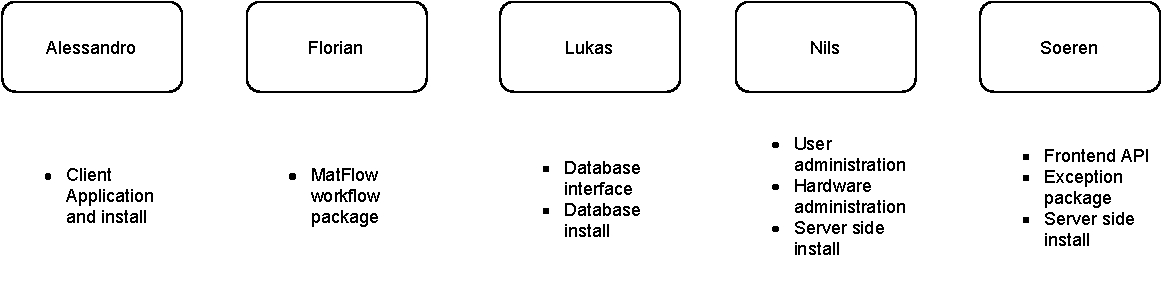
\includegraphics[scale=0.8]{res/aufteilung.pdf}}
    \caption{Aufteilung}
    \end{figure}

\subsection{Endgültiger Stand nach Implementierung}
Frontend
\begin{itemize}
    \item \textbf{Jede} der anzuwählenden Seiten ist implementiert
    \item Alle benötigten Datenklassen sind voll funktionsfähig implementiert
\end{itemize}
Frotend API
\begin{itemize}
    \item \textbf{Jede} der zur Verfügung stehenden Methoden ist bis auf die \nameref{Cookie} voll funktionsfähig implementiert
    \item Alle Unit Tests sind geschrieben
\end{itemize}
User Administration
\begin{itemize}
    \item \textbf{Jede} der zur Verfügung stehenden Methoden ist voll funktionsfähig implementiert
    \item Alle Unit Tests sind geschrieben
\end{itemize}
Hardware Administration
\begin{itemize}
    \item \textbf{Jede} der zur Verfügung stehenden Methoden ist voll funktionsfähig implementiert
    \item Alle Unit Tests sind geschrieben
\end{itemize}
Workflow Package
\begin{itemize}
    \item \textbf{Jede} der zur Verfügung stehenden Methoden ist voll funktionsfähig implementiert
    \item Alle Unit Tests sind geschrieben
\end{itemize}
Exception package
\begin{itemize}
    \item \textbf{Jede} der zur Verfügung stehenden Methoden ist voll funktionsfähig implementiert
\end{itemize}
Database package
\begin{itemize}
    \item Der Großteil der zur Verfügung stehenden Methoden ist voll funktionsfähig implementiert
    \item Alle Unit Tests sind geschrieben
\end{itemize}
Zu implementieren bleibt noch
\begin{itemize}
    \item Die request Klasse BackendCommunicator und Unit Tests im Frontend
    \item Die WorkflowData Schnittstelle im Database package
    \item Der alternierende Operator für airflow
    \item Die containerweise Ausführung der Serverapplikation im Backend (Nomad Job File)
\end{itemize}
\section{Entwurfsumentscheidungen}
    	
  
\subsection{Memento} 	
    	 The memento pattern is used to set a view to the default state. Every view has its default
    	 state that is created at the start of the view. When a user makes an input, the view and
    	 its state changes. Whenever a user sends a request to the backend-server, the view should
    	 be reset, so that no mistakes are made on future requests. The memento pattern comes in
    	 place and sets the default state of the view and the view displays it accordingly. In
    	 the future it would be possible to safe inputs and load them as the view's new state.
    	\begin{figure}[H]
            \label{API}
            \centerline{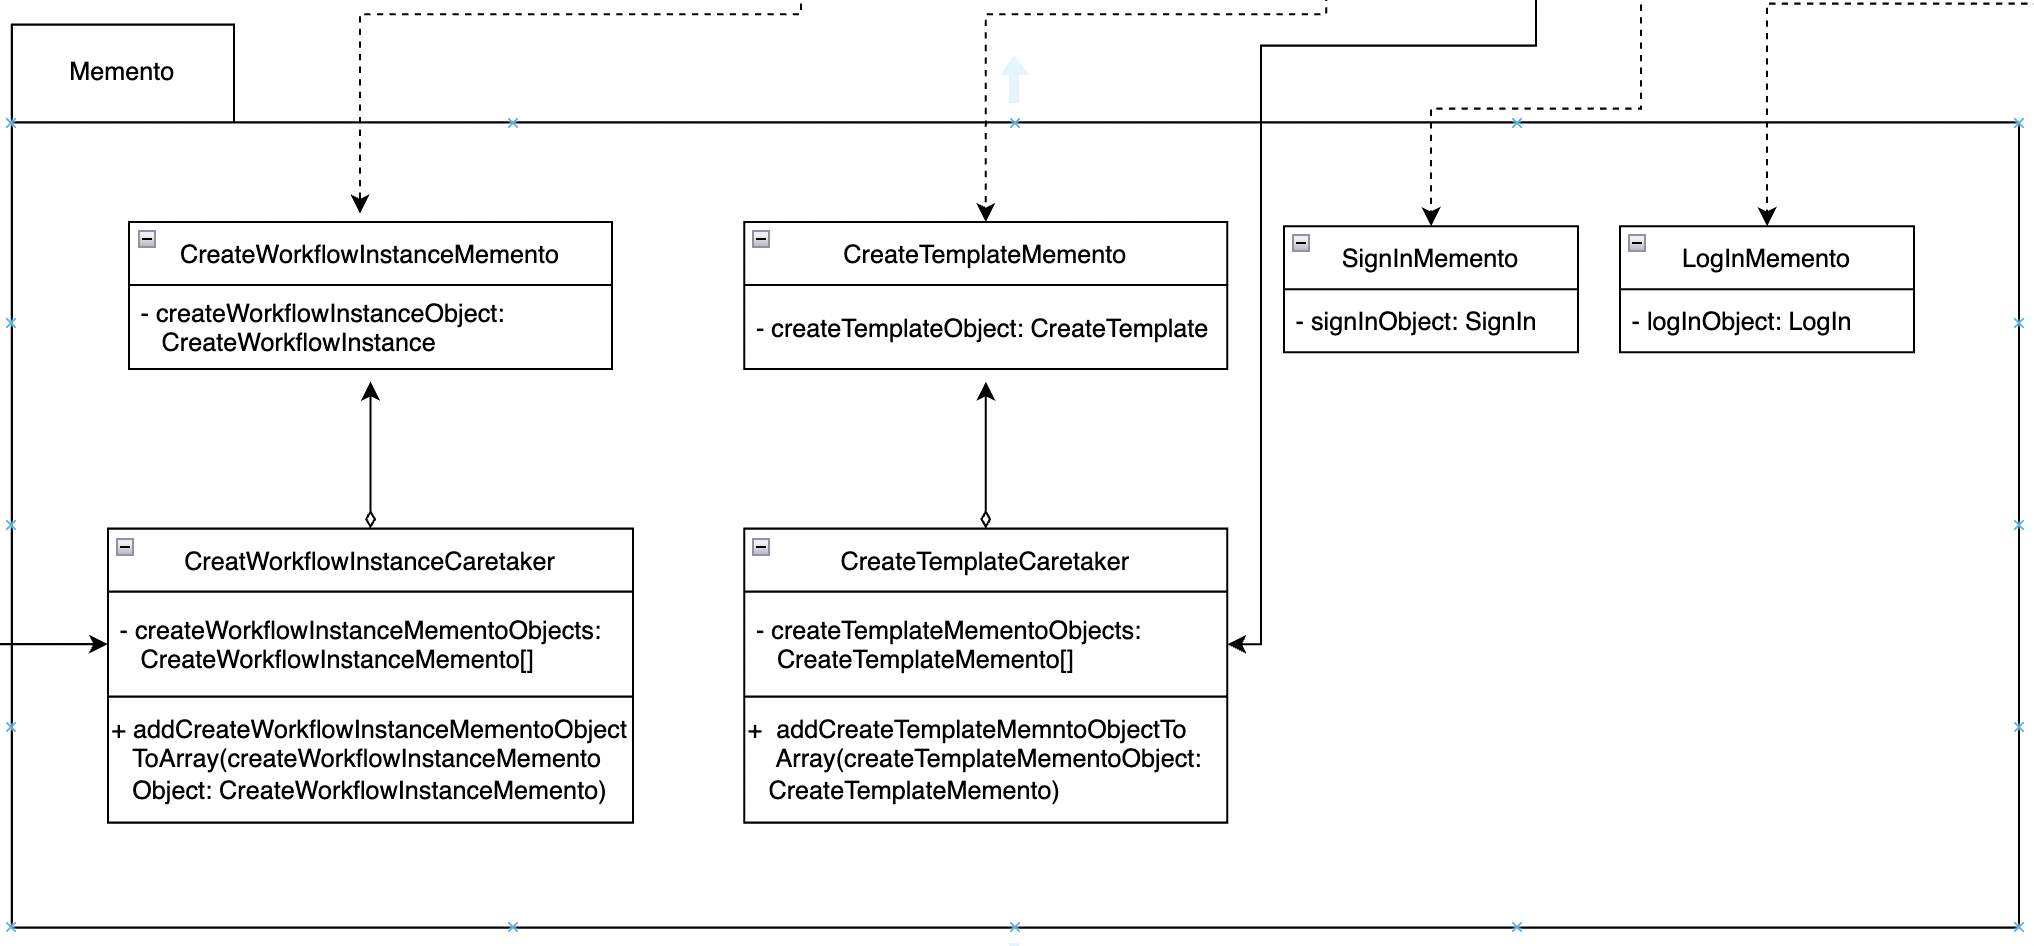
\includegraphics[scale=0.5]{res/Memento.png}}
            \caption{Memento package}
    	\end{figure}
    	\newpage
    	
\subsection{JSON Converter}
    \subsubsection{Frontend}
    	A controler handels every request to convert a JSON-object into a class object.
    	The controler takes in a string with the classname and the JSON-object, calls the 
    	method create...ObjectFromJSON in the corresponding class and returns the created object. 
    	\begin{figure}[H]
            \label{API}
            \centerline{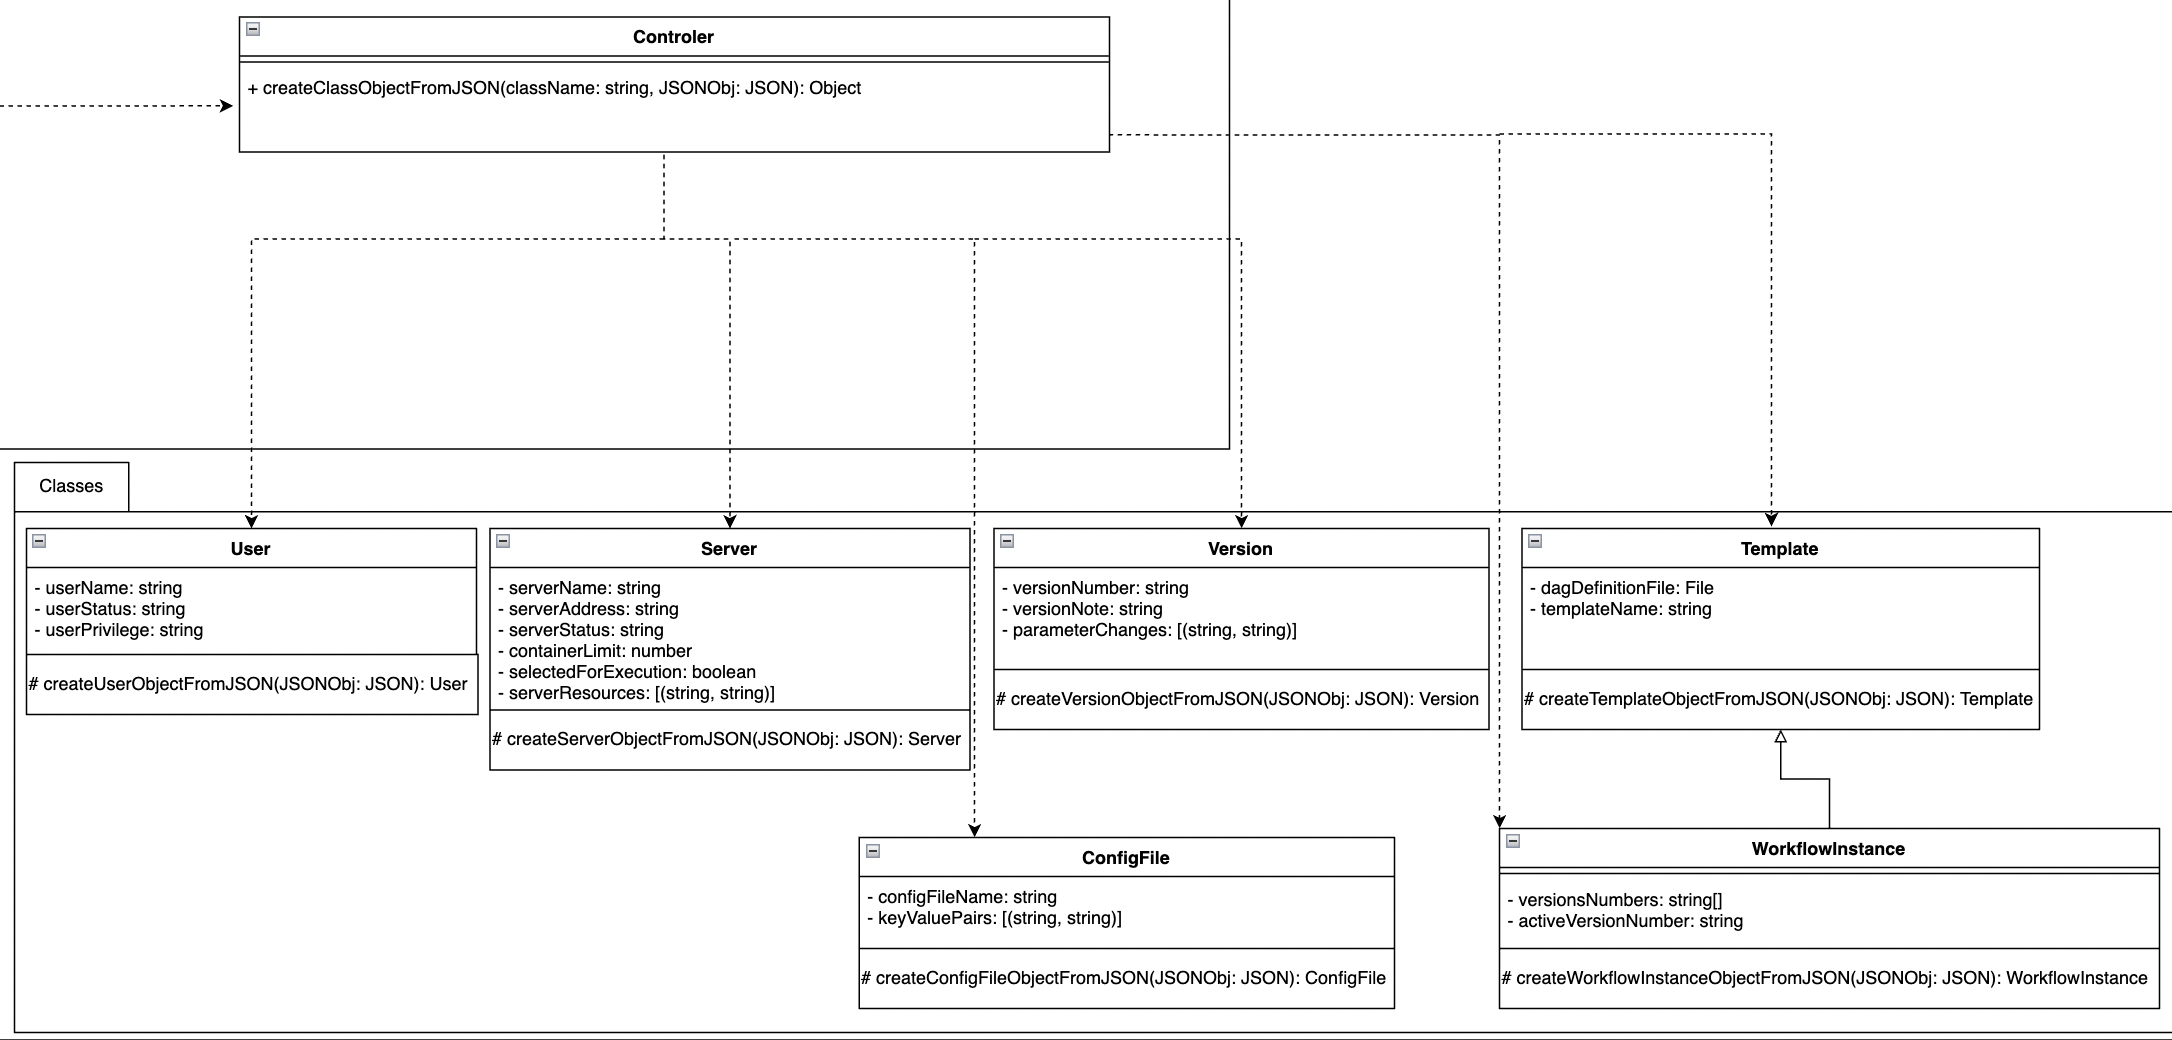
\includegraphics[scale=0.5]{res/Controler.png}}
            \caption{Controler package}
    	\end{figure}
    \subsubsection{API} \label{json_backend}
        \begin{figure}[H]
            \label{API}
            \centerline{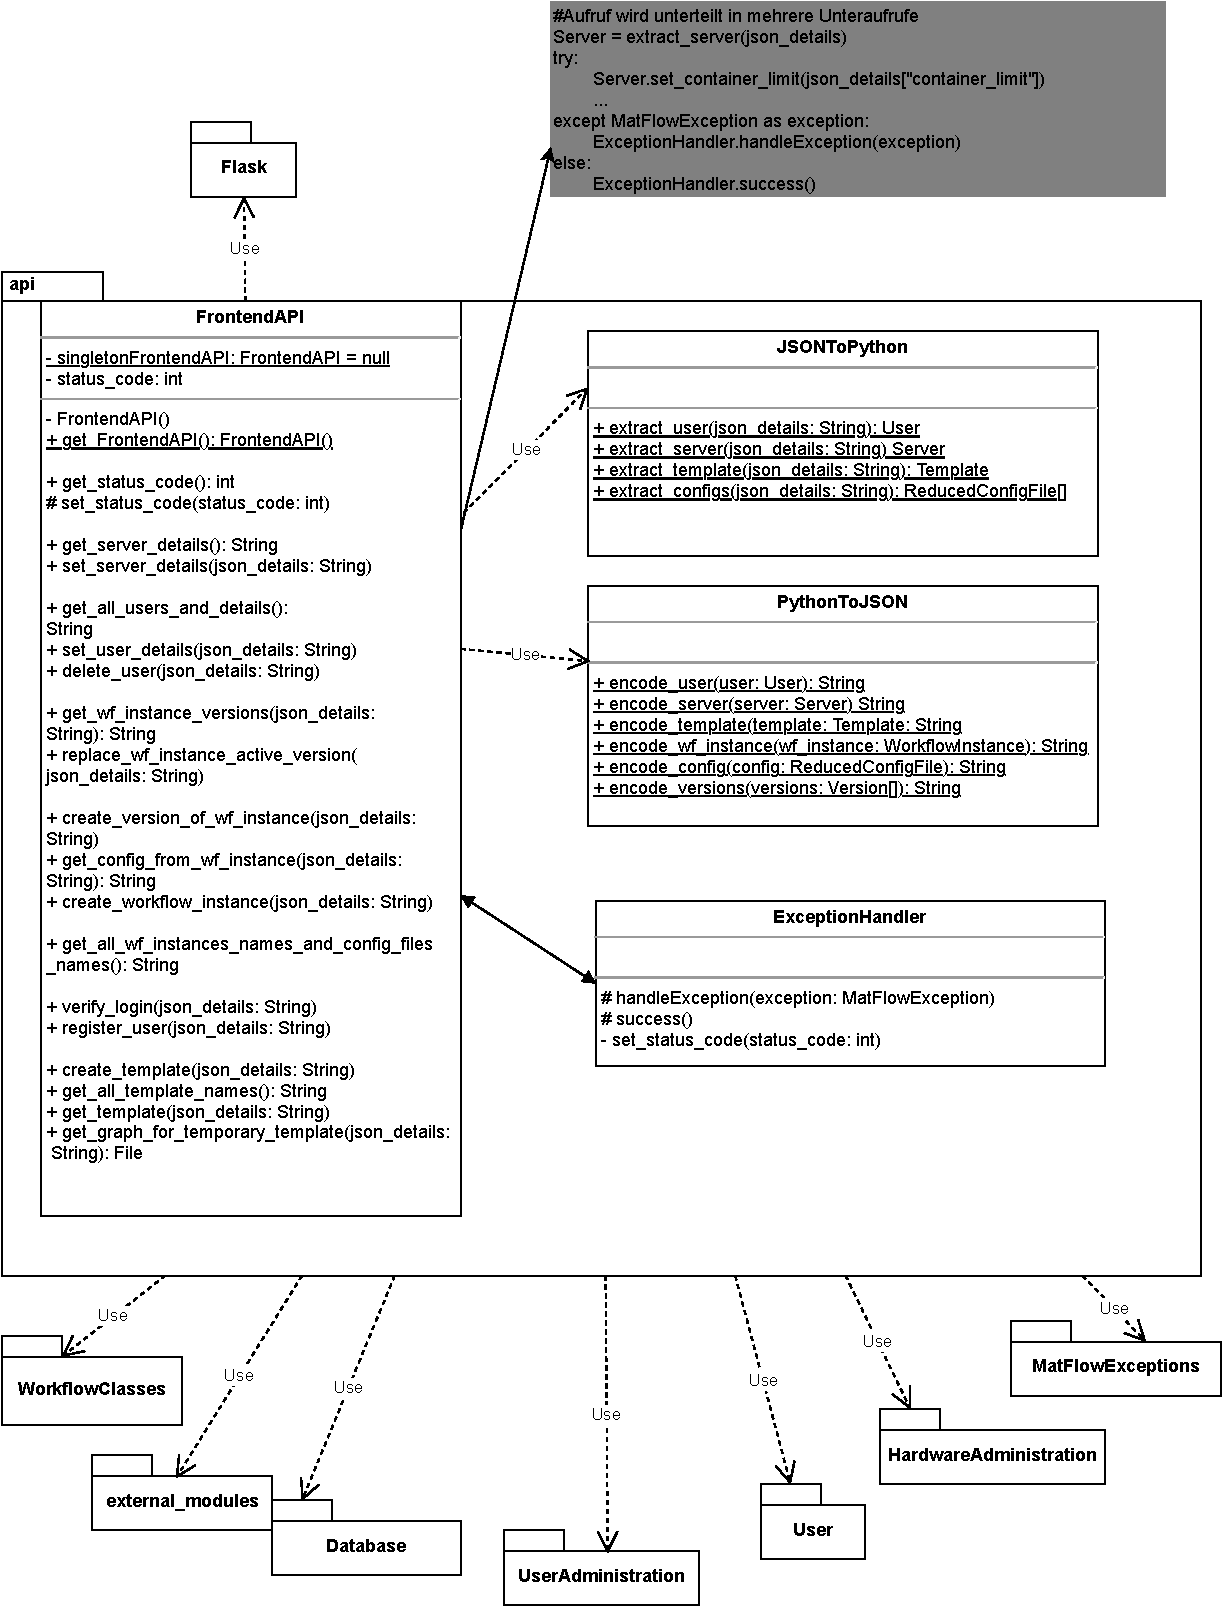
\includegraphics[scale=0.5]{res/api.drawio.pdf}}
            \caption{API package}
        \end{figure}
        \vspace{0.3in}
        Im Backend sind auch analog zum Frontend zwei JSON Converter(jewils von und zu) vorhanden.
        Diese Entwurfsentscheidung wurde aber verworfen, da sie das Kapselungsprinzip verletzt.
        Von nun an sind alle in den Converter vorhandenen Methoden direkt als Klassen- (von JSON)
        oder Objektmethoden (zu JSON) direkt in den jeweiligen Klassen implementiert. Als Beispiel: 
        encode\texttt{\_}template(template: Template) und extract\texttt{\_}template(json\texttt{\_}details: String): Template
        sind nun als encode\texttt{\_}template(self): str und \texttt{\@}classmethod extract\texttt{\_}template: Template 
        in Template vorhanden.    


\subsection{JSON Status Code}
Wie man auch in der \nameref{API} sieht, ist die Bereitstellung eines Status Codes bei einem request an die API nicht eindeutig
dem Entwurf zu entnehmen, deswegen hier noch einmal eine saubere Erläuterung:
Es wird bei einer Anfrage an die API diese Anfrage durchgeführt. Je nachdem ob sie nicht erfolgreich war (MatFlowException 
geworfen, spezieller Status Code vorhanden) oder doch erfolgreich war (success Status Code und eventuell Daten vorhanden) 
wird in der Klasse ExceptionHandler die Antwort in json gebaut und an den Client zurück geschickt. 
Der Client bekommt also \textbf{immer} eine Antwort mit einem json response body, indem sich der status code befindet. 
Es handelt sich hier also nur um eine Anlehnung an die bereits etablierten HTTP Status Codes.

\subsection{Authentifizierung} \label{Cookie}
Im Frontend kann man theoretisch unabhängig der User Privilegien mittels URL Manipulation auf alle 
Seiten zugreifen. Um dies zu verhindern, wird im Frontend ein einzigartiges Cookie mit der Anfrage an die Frontend
API geschickt, die dann ??
% TODO Alessandro
% TODO Nils dann Entwurf ändern und neues Bild posten
\subsection{Entfernen der Login und SignUp Klasse}
Während der Implementierung der UserAdministration, ist schnell aufgefallen, dass sowohl Login- als auch SignUp keine benötigten Klassen sind.
Stattdessen ist die Logik von Login und SignUp nun in der UserController Klasse beinhaltet.

\begin{figure}[h]
            \label{UserAdministration}
            \centerline{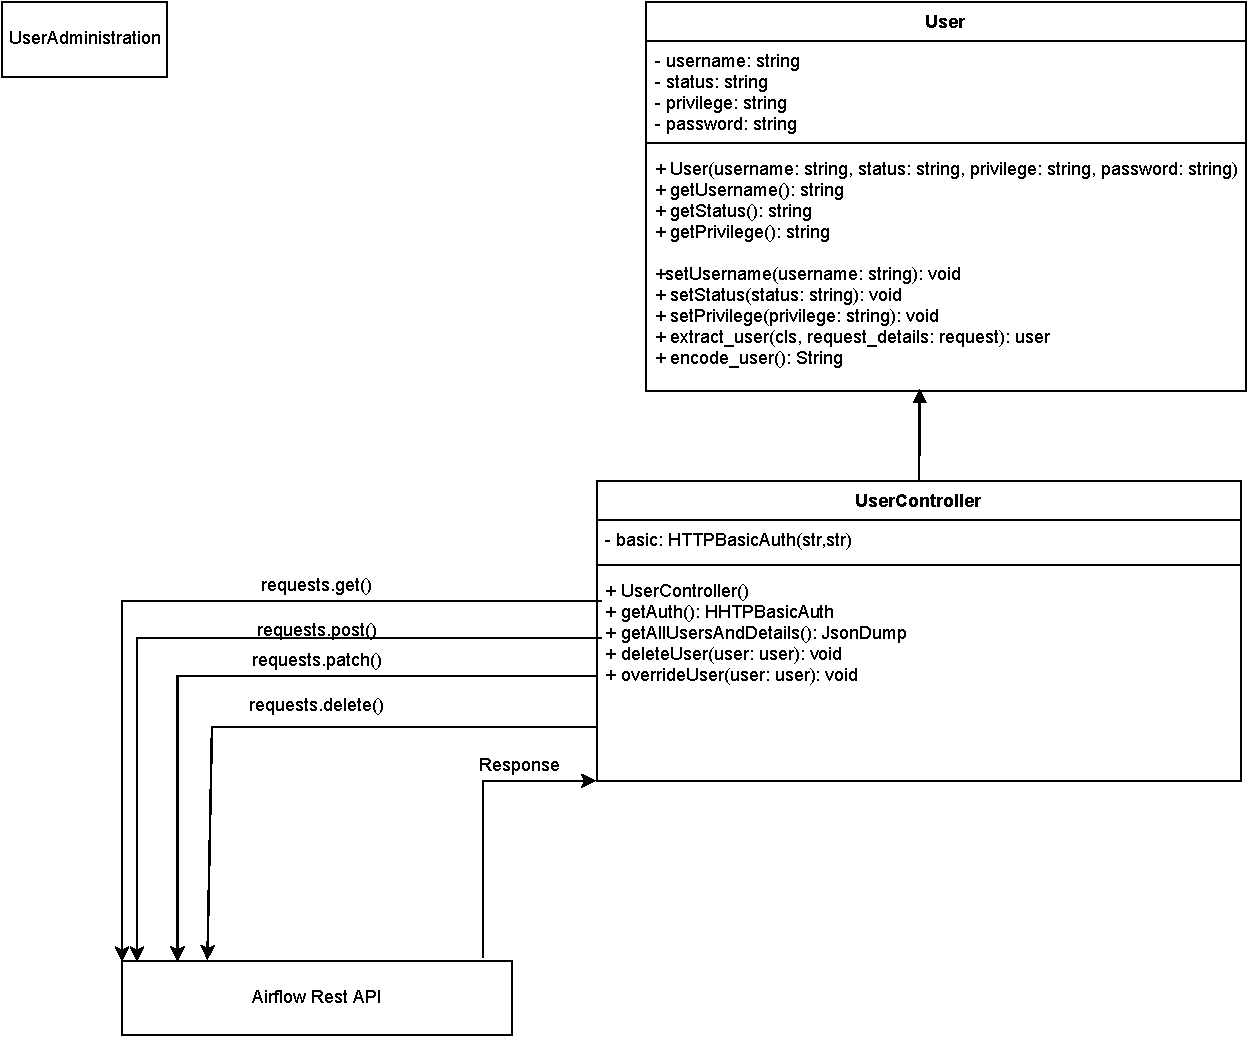
\includegraphics[scale=0.7]{res/UserAdministration.pdf}}
            \caption{Die überarbeitete Version der UserAdministration}
\end{figure}

In dem Diagramm wurden die 2 Redundanten Klassen entfernt und neue Methoden hinzugefügt. Des Weiteren ist die Schnittstelle zu Airflow nun genauer definiert worden.
\subsection{hinzufügen der Schnittstelle zur Datenbank}
Der Entwurf der HardwareAdministration konnte gut umgesetzt werden. Jedoch musste eine Schnittstelle zur Datenbank hinzugefügt werden, da der/die Server nicht über Airflow reguliert
werden konnten.

\begin{figure}[h]
            \label{HardwareAdministration}
            \centerline{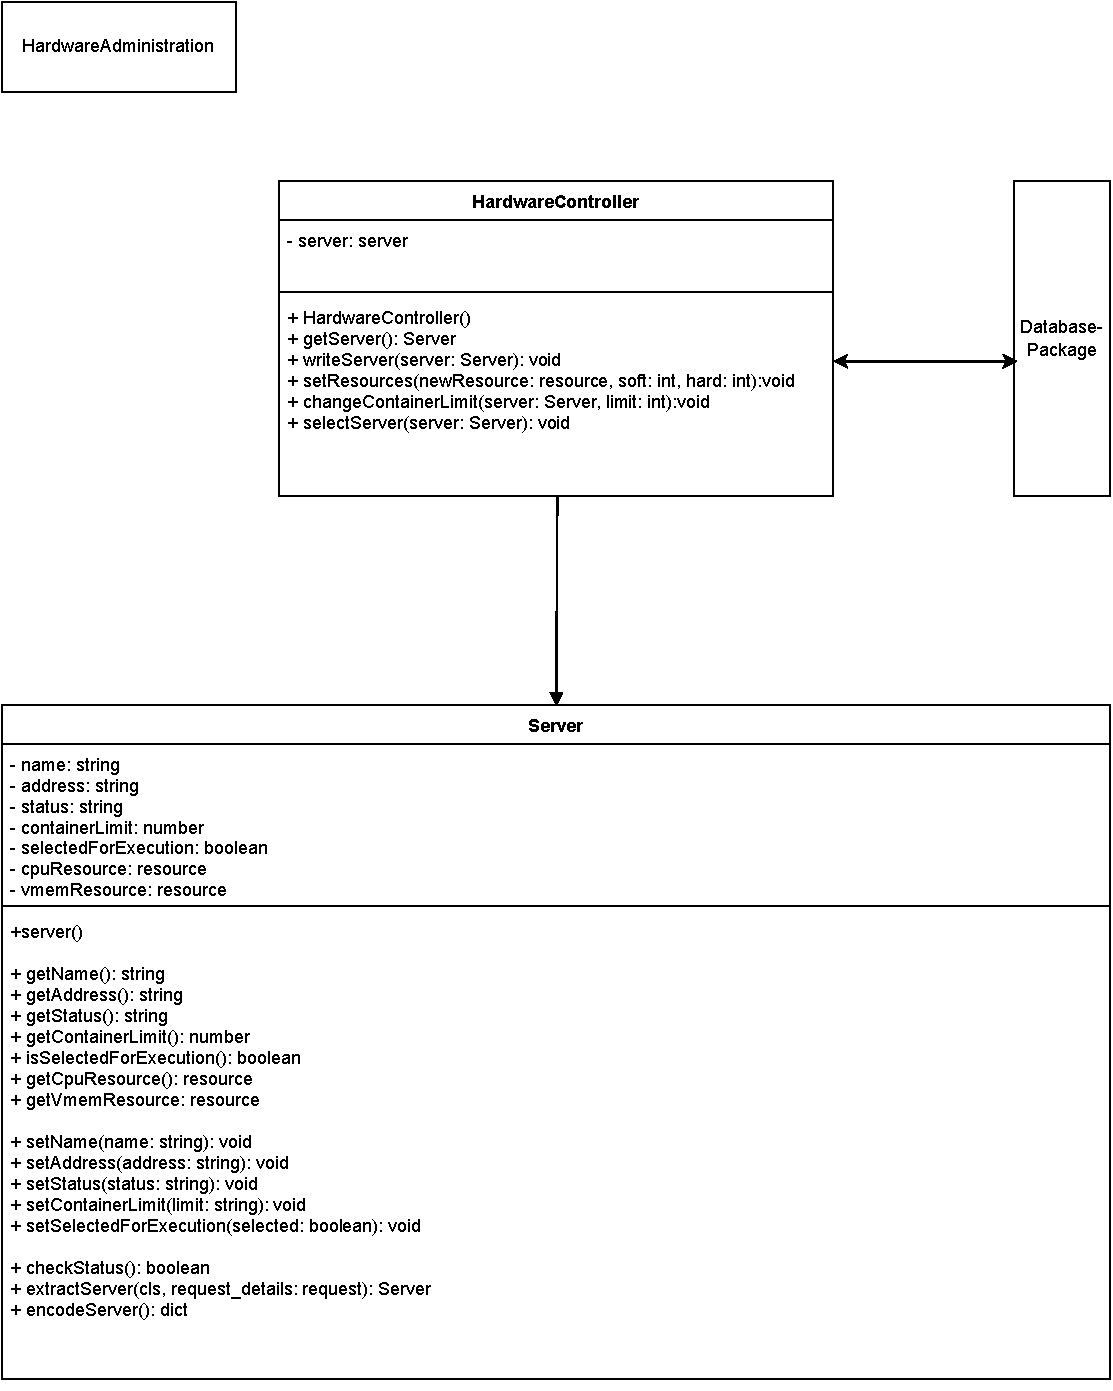
\includegraphics[scale=0.7]{res/HardwareAdministration.pdf}}
            \caption{Die überarbeitete Version der HardwareAdministration}
\end{figure}

In dem Diagramm wurden ein paar Methoden und die Schnittstelle zur Datenbank hinzugefügt.



%TODO an alle: Entwurfsänderungen hinzufügen
\subsection{Kommunikation von Dateien innerhalb der Serveranwendung}
Alle Attribute, Parameter und Rückgaben, die im Entwurfsheft mit dem Typ "File" gekennzeichnet waren, haben wir jetzt als "Path" implementiert. Wobei wir die Klasse "Path" aus dem Modul "pathlib" der Python-Standardbibliothek importieren.

Im Folgenden soll die Handhabung der Dateien unter Zuhilfenahme von Pfaden erklärt werden. Dateien, die durch die API die oberste Schicht der Serverandwendung erreichen werden zunächst in einem temporären Ordner zwischen gespeichert. Der entsprechende Pfad im temporären Ordner wird entweder durch Aufruf eines Konstruktors in einem Objekt abgelegt oder unmittelbar an die Schnittstelle des Workflow-Packages übergeben.
Dort wird der Datei dann dem Aufruf entsprechend ein langfristiger Speicherort im Dateisystem zugewiesen. Die Löschung der Dateien im temporären Ordner obliegt dem Empfänger. Muss umgekehrt eine Datei vom Workflow-Package an die Schnittstelle der Serveranwendung gealngen, so wird der Pfad des langfristigen Speicherorts verwendet. Dort kann die Datei ausgelesen werden, gelöscht wird sie anschließend natürlich nicht.

Im Entwurfsheft haben wir uns keine Gedanken über die Ordnerstruktur der auf dem Server gespeicherten Dateien gemacht, deshalb reichen wir nun einen entsprechenden Entwurf nach. 

\subsection{Änderungen im Workflow-Package} % Florian
% ich werde hier in meiner externen file die subsections "Kommunikation von Dateien innerhalb der Serveranwendung" und "Änderungen im Workflow-Package" hinzufügen. Im ersteren Kapitel würde ich auch die von meinem package angelegte und verwaltete File-System-Struktur erklären. Nur damit sich das nicht zu sehr mit Lukas Text überschneidet


%\subsection{MySQL - Datenbankaufbau}

\begin{figure}[h]
	\centering
	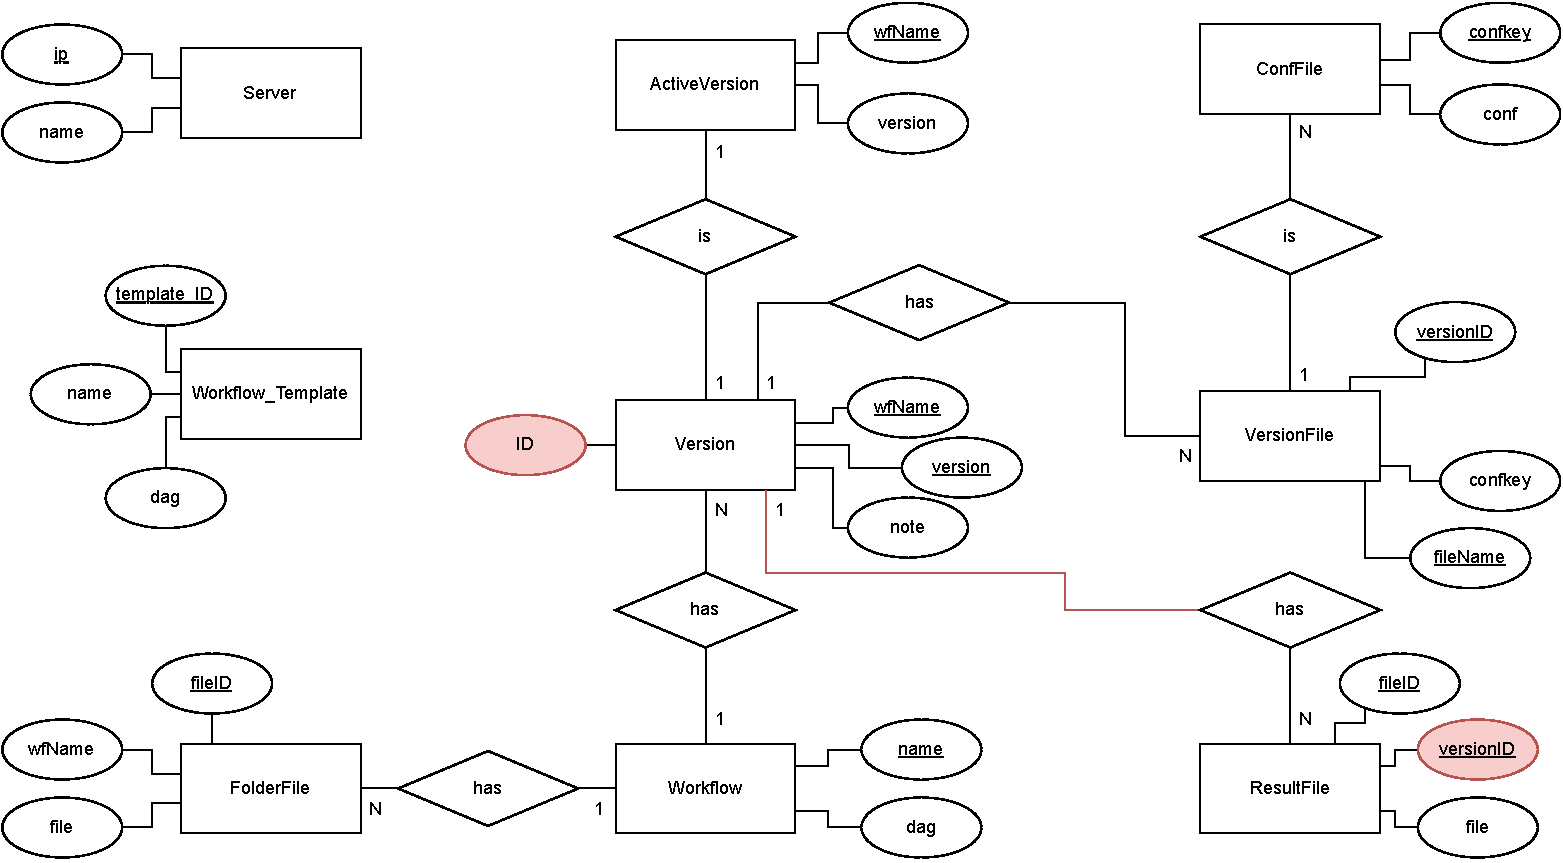
\includegraphics[width=0.85\textwidth]{res/er_diagram.pdf} 
	\caption{ER-Diagramm der Datenbank; überarbeitet\\ Änderungen in rot}
	\label{fig:er_diagram}
\end{figure}

Auf \ref{fig:er_diagram} ist das Überarbeitete ER-Diagramm der Datenbank zu sehen.

Nach langen Überlegungen sind wir zu dem Schluss gekommen, dass es sinnvoller ist für die Dateispeicherung statt LONGBLOBS und weitere Parameter, nur Pfade in die Datenbank einzuspeichern, die auf die gewünschte Datei zeigen. Zum einen gibt es dadurch weniger rohe Daten die zwischen (manchen) Funktionen kommuniziert werden müssen, aber auch weniger Latenz beim schreiben oder lesen der Dateien aus der Datenbank.

Weitere Änderungen beinhalten die Vereinfachung einer Workflow-Version in der Datenbank. Statt zwei Schlüssel 'wfName' und 'version' bekommt jede Version einen eindeutigen Integer Bezeichner. Dieser muss zwar für manche Zugriffe auf andere Tabellen zuerst von Version geholt werden, erhöht aber das Verständnis der Datenbankstruktur und bringt eine Erleichterung der MySQL-Befehle.

Die Verbindung von ResultFile wurde außerdem zu Version geändert. Es besteht keinen Grund das komplexe System der Speicherung von überlappenden .conf Dateien auch für die (höchstwahrscheinlich) immer unterschiedlichen Ergebnisse unterschiedlicher Versionen zu nutzen. Ein einfacher Fremdschlüssel der auf die entsprechende Workflow-Version zeigt reicht aus.


Dementsprechend sind Folgende Tabellen in der Datenbank vorhanden:

\paragraph{}
\begin{dataTable}
	\hline
	\textbf{Server} & & \\
	\hline
	ip & varchar(50) & $key$ \\
	\hline
	name & varchar(255) & $key$ \\
	\hline
\end{dataTable}

\paragraph{}
\begin{dataTable}
	\hline
	\textbf{WorkflowTemplate} &  & \\
	\hline
	template\textunderscore ID & int & $key; Auto_Increment$\\
	\hline
	name & varchar(255) & $notNull$ \\
	\hline
	dag & varchar(255) & $notNull$\\
	\hline
\end{dataTable}

\paragraph{}
\begin{dataTable}
	\hline
	\textbf{Workflow} &  & \\
	\hline
	name & varchar(255) & $key$ \\
	\hline
	dag & varchar(255) & $notNull$\\
	\hline
\end{dataTable}

\paragraph{}
\begin{dataTable}
	\hline
	\textbf{FolderFile} &  & \\
	\hline
	filesID & int & $key; Auto_Increment$ \\
	\hline
	wfname & varchar(255) & $notNull;$ name from Workflow\\
	\hline
	file & varchar(255) & $notNull$\\
	\hline
\end{dataTable}

\paragraph{}
\begin{dataTable}
	\hline
	\textbf{Version} & & \\
	\hline
	ID & int & $key; Auto_Increment$ \\
	\hline
	wfName & varchar(255) & name from Workflow\\
	\hline
	version & varchar(127) & $notNull$ \\
	\hline
	note & varchar(1000) & \\
	\hline
\end{dataTable}

\paragraph{}
\begin{dataTable}
	\hline
	\textbf{ActiveVersion} & & \\
	\hline
	wfName & varchar(255) & $key;$ name from Workflow\\
	\hline
	version & varchar(127) &  from Version\\
	\hline
\end{dataTable}

\paragraph{}
\begin{dataTable}
	\hline
	\textbf{VersionFile} & & \\
	\hline
	versionID & int & $key;$ ID from Version \\
	\hline
	filename & varchar(255) & $key$\\
	\hline
	confKey & int & $notNull;$ from ConfFiles \\
	\hline
\end{dataTable}

\paragraph{}
\begin{dataTable}
	\hline
	\textbf{ConfFile} & & \\
	\hline
	confKey & int & $key; Auto_Increment$ \\
	\hline
	file & varchar(255) & $notNull$ \\
	\hline
\end{dataTable}

\paragraph{}
\begin{dataTable}
	\hline
	\textbf{ResultFile} &  & \\
	\hline
	versionID & int & $key;$ ID from Version \\
	\hline
	filesID & int & $key; Auto_Increment$ \\
	\hline
	file & varchar(255) & $notNull$\\
	\hline
\end{dataTable}



\subsection{Database Paket Implementierungsänderungen} %Lukas
\section{Anhang}\label{Anhang}
\subsection{Detailliertere Aufteilung}
Man sieht im Folgenden die exportierten Issues aus Gitlab:
\begin{figure}[H]
    \centerline{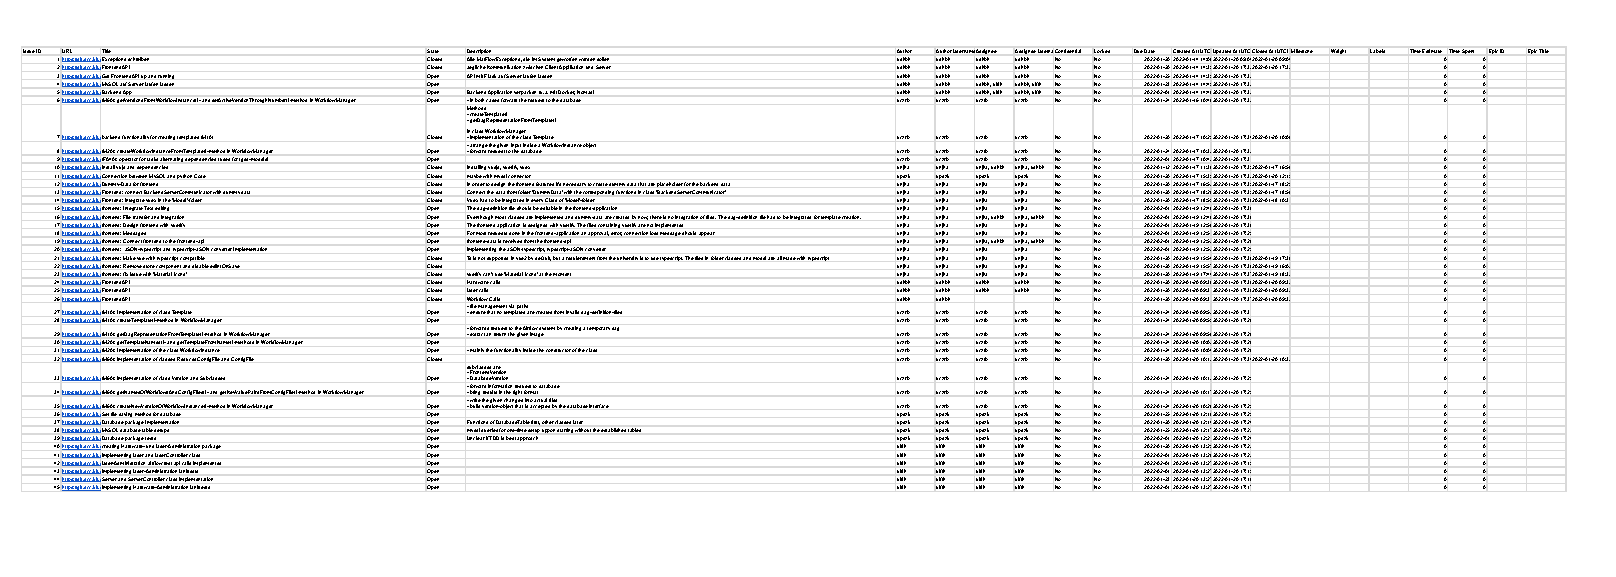
\includegraphics[scale= 0.7]{res/daniel_aufteilung_cropped.pdf}}
    \caption{Aufteilung}
    \end{figure}
\pagebreak
% Glossar
\clearpage
%\printnoidxglossaries

\end{document}